%\documentclass[jkps,preprint,fleqn,showpacs,showkeys]{revtex4}
\documentclass[jkps,fleqn,showpacs,showkeys]{revtex4}
\usepackage[pdftex]{graphicx}
\usepackage{amssymb}
\usepackage[dvipsnames]{xcolor}
\usepackage{amsmath}
\usepackage{bm}
\usepackage{tabularx}


\usepackage{kotex}


\begin{document}
\newcolumntype{C}[1]{>{\centering\arraybackslash}p{#1}}


\setcounter{page}{1}
\title[]{Analysis of the near-side Ridge in high-multiplicity pp collisions \\ via Momentum-Kick model}
\author{Jaesung \surname{Kim}}
\author{Jin-Hee \surname{Yoon}}
\email{jinyoon@inha.ac.kr}
% \thanks{Fax: +82-2-6490-5750}
\affiliation{Department of physics, Inha University, Incheon 402-751}
\date[]{Received !Month !day 2022}

\pacs{}
\keywords{Oh My God!}


\begin{abstract}
The near-side ridge structure was observed at the long-range in the two-particle correlations, which is observed in heavy-ion collisions like AuAu collision at the Relativistic Heavy Ion Collider (RHIC), PbPb and pPb collisions at the Large Hadron Collider(LHC).
The ridge structure in the heavy-ion collisions could be understood by hydrodynamic models.
However, the ridge structure is also observed in a small-system, which is observed in the proton-proton collision at the LHC experiments.
Since the small system creates a lower density than heavy-ion collisions, we assume that the effect of kinematics is increased.
The Momentum-Kick model is based on kinematics, which explains the ridge structure as kicked medium partons by jet particles.
Therefore, we expect that the Momentum-Kick model can explain proton-proton collision in various momentum at 13TeV in the LHC.
We already know that the Momentum-Kick model makes clear the near-side ridge structure in the proton-proton collision.
Therefore, we check whether the Momentum-Kick model applies to various momentum, we conclude the Momentum-Kick model can describe the ridge structure well in diverse momentum, and we need to further study for various energy and multiplicity cuts.
\end{abstract}


\maketitle

\section*{INTRODUCTION}
\label{sec:Introduction}

The ridge structure refers to the shape of ‘ridge’ in the $\Delta\eta - \Delta\phi$ correlation that appears at long-range.
Previously, the ridge structure was observed in the case of heavy-ion collisions such as AuAu collisions at the Relativistic Heavy Ion Collider (RHIC) \cite{ref12, ref13, ref14, ref15, ref16, ref17, ref18, ref19, ref20, ref21, ref22, ref23, ref24, ref25, ref26, ref27}, and PbPb at the Large Hadron Collider (LHC) \cite{ref1, ref2, ref3, ref4, ref5, ref6, ref7, ref8, ref9, ref10, ref11}.
In these cases, the ridge structure can be understood by collective motion, based on hydrodynamics theory, because it is enough to create high-temperature and high-density environment.
And this is the hint of Quark-Gluon Plasma (QGP) state.
Recently, however, the ridge structure is also observed in the high multiplicity of the proton-proton collision, which is the small system.
It was expected that the small system could not create an environment like heavy-ion collisions, and the medium doesn't make the collective motion.

The Momentum-Kick model\cite{Wong_2, Wong_3, Wong_4, Wong_5} is based on pure kinematics between near-side jet and medium partons, which assumes that the medium particles are kicked by near-side jet particles, and the kicked partons make a collective motion, like heavy-ion collision.
Since the Momentum-Kick model is successfully applying the experimental results in AuAu at 200 GeV\cite{Wong_1}, PbPb at 2.76 TeV\cite{PbPb}, and pp at 13 TeV\cite{Hanul}, we expect that the model can explain well ridge structure at the various momentum in high multiplicity small system.
We describe the various momentum in proton-proton collisions, which is a further step from the previous proton-proton at 13TeV results\cite{Hanul}, using the same $f_R \langle N_k \rangle$ form in the previous PbPb at 2.76TeV results\cite{PbPb}.
Therefore, we will analyze the high multiplicity proton-proton collision at 13 TeV from A Large Ion Collider Experiment (ALICE), Compact Muon Solenoid (CMS), and A Toroidal LHC Apparatus (ATLAS) experiments via the Momentum-Kick model\cite{alice,cms,atlas}.

\section*{Momentum-Kick Model}
\label{sec:Momentum-Kick Model}

The Momentum-Kick model explains the results of experiments at the near-side region, through the behavior of near-side jet fragments kicking the medium partons.
The kicked medium partons make the collective motion, which is the reason for the near-side ridge structure.
Since the small system create lower density of the medium particles, we expect that kinematics behavior is more dominant in the small system than heavy-ion collisions.
Hence, the Momentum-Kick model will be expected to describe successfully in proton-proton collision at 13TeV in high-multiplicity.


Since the near-side jet fragments usually distribute at short-range and the pp at 13TeV data have only long-range and near-side data, we use only the ridge component and it is expressed as:
\begin{equation} \label{equation:eq1}
\frac{2}{3} f_R\left\langle N_k\right\rangle \frac{dF}{p_T dp_T d\Delta\eta d\Delta\phi},
\end{equation}
where $\Delta \eta $ and $\Delta \phi$ are the differences of $\eta$ and $\phi$ between jet and the other particles, $f_R$ is the average survival factor of ridge particles, and $\left\langle N_k\right\rangle$ is the average of kicked partons per-trigger particle.

The Momentum-Kick model explains the ridge component via soft scattering model as follows:
\begin{equation} \label{equation:eq4}
\frac{dF}{p_Tdp_Td\eta d\phi}
= \left[\frac{dF}{p_{Ti}dp_{Ti}dy_id\phi_i} \frac{E}{E_i} \right]_{\mathbf{p}_i=\mathbf{p}-\mathbf{q}}\times\sqrt{1-\frac{m^2}{\left(m^2+p_T^2\right){\cosh}^2y}}.
\end{equation}
$ dF / p_{Ti}dp_{Ti}dy_id\phi_i $ is the normalized initial parton distribution, which implies the distribution before freezing out.
$\mathbf{p}_i$ is the initial parton momentum, and $\mathbf{p}$ is the momentum of the final parton after the kicked as $\mathbf{q}$.
Since the most of the near-side jet is concentrated in the perpendicular direction of beam axis, the transverse momentum of initial particles is written as follows:
\begin{equation} \label{equation:eq5}
p_{Ti}^2=p_{T}^2-2p_{T} q \cos\left(\Delta\phi\right)+q^2.
\end{equation}
% $\Delta\eta,\Delta\phi \sim 0$ region, we set $\eta_{\text{jet}}=0$.
$E/E_i$ insures conservation of energy between initial and final partons.
$\sqrt{ \left. 1- m^2 \middle/ \left(m^2+p_T^2\right){\cosh}^2y \right.}$ converts the rapidity into pseudo-rapidity.

The initial parton momentum distribution is expressed as follows:
\begin{equation} \label{equation:eq6}
\frac{dF}{p_{Ti}dp_{Ti}dy_id\phi_i}=A_{\text{ridge}}\left(1-x\right)^a\frac{e^{ \left. -\sqrt{m^2+p_{Ti}^2} \middle/ T \right. }}{\sqrt{m_d^2+p_{Ti}^2}},
\end{equation}
where $A_{\text{ridge}}$ is the normalization constant.
$T$ is one of the major parameters to explain momentum distribution, indicating the temperature of medium particles.
Since pions are expected to take up the majority of partons, we set $m$ as the mass of the pion, which $m$ means the medium parton mass.
$m_d$ is a cut-off parameter that prevents divergence at small $p_{Ti}$.
$a$ is a fall-off parameter, which determines the rate of decrease of $1-x$ distribution.
$m_d$ and $a$ are set the same as references\cite{PbPb, Wong_1}, which we take $m_d = 1.0$GeV and $a = 0.5$, for the general application of the Momentum-Kick model\cite{Wong_1}.
Also, $x$ is the light-cone variable written as follows:
\begin{equation} \label{equation:eq8}
x=\frac{\sqrt{m^2+p_{Ti}^2}}{m}e^{\left|y_i\right|-y_b},
\end{equation}
where $y_b$ is the rapidity of the beam defined as $y_b=\cosh^{-1}{\sqrt{s_\text{NN}}/2m_N}$. $m_N$ is the mass of beam particles, set as the proton mass.


\section*{FITTING RESULTS}
\label{sec:Fitting results}

\subsection{Experimental environment}
\label{subsec:Experimental environment}

We verify our model in ALICE, CMS and ATLAS experiments\cite{alice,cms,atlas} via least square method.
The conditions of data analyzed in these experiments are summarized in Table \ref{table:range}.
In the case of $\Delta\eta$ range, ALICE experiment is narrower than CMS and ATLAS.
Also, ALICE experiment defines the high multiplicity as the top $0\sim0.1\%$ multiplicity, which is distinct from other experiments in that they define the range of multiplicity.
And, ALICE and CMS experiments split their data as $p_T$ range.

\begin{table}[ht]
  \centering
  \begin{tabular}{C{3cm} | C{3cm}  C{3cm}  C{3cm} } 
  \hline \\[-1 ex]
   & ALICE & CMS & ATLAS \\ [1 ex] \hline\hline \\[-1.5ex]
  $\Delta \eta $ range & $1.6<|\Delta \eta |<1.8$ & $2<|\Delta \eta |<4$ & $2<|\Delta \eta |<5$ \\ [1ex] 
  Multiplicity & $0\sim0.1\%$ & $N_{\text{trk}}^{\text{offline}} \geq 105$ & $N_{\text{ch}}^{\text{rec}} \geq 90$ \\[1ex] 
  $p_T$ range & $1<p_T<4$ & $0.1<p_T<4$ & $0.5<p_T<5$ \\[1 ex]
  \hline
 \end{tabular}
 \caption{The ranges of data in ALICE, CMS, and ATLAS experiments\cite{alice, cms, atlas}}
 \label{table:range}
\end{table}

Moreover, all three results used different analyzing methods.
In ALICE and CMS analysis, they used Zero Yield At Minimum (ZYAM) method, a traditional experimental analysis method.
In this method, the minimum value is set to zero by subtracting.
However, ATLAS used the peripheral subtraction method.
It takes the ridge component from the experiment data by subtracting the peripheral component, which is low multiplicity pp collisions, to check the flow effect.
Therefore, we apply ZYAM method when we use ATLAS experiment data for consistency.

\subsection{Does $f_R\langle N_k \rangle$ have $p_T$ dependence?}
\label{subsec: pT depnedence}

Since the initial parton momentum distribution is normalized, $f_R\langle N_k \rangle$ describe the number of particles, which survives and is detected at the detector.
We set $f_R\langle N_k \rangle = Ae^{-{B} / p_T -C p_{T}}$ form (A, B, and C are positive real number), which is the same $f_R\langle N_k \rangle$ form in PbPb at 2.76TeV result\cite{PbPb}.
So, we need to check $f_R\langle N_k \rangle = Ae^{-{B} / p_T -C p_{T}}$ form.
However, the least square method via the Levenberg-Marquardt algorithm eliminates $e^{-Cp_T}$ term.
And the $e^{-B/p_T}$ term only effect at the $0.1<p_T<1$GeV range, which has high fluctuation and low statistics data.
Therefore, we also check $f_R\langle N_k \rangle$ as constant, and Fig\ref{figure:ptVSnone} is a graph compared the fitting result of $f_R\langle N_k \rangle$ as $Ae^{-{B} / p_T -C p_{T}}$ form and constant.

\begin{figure}[ht]
\centering
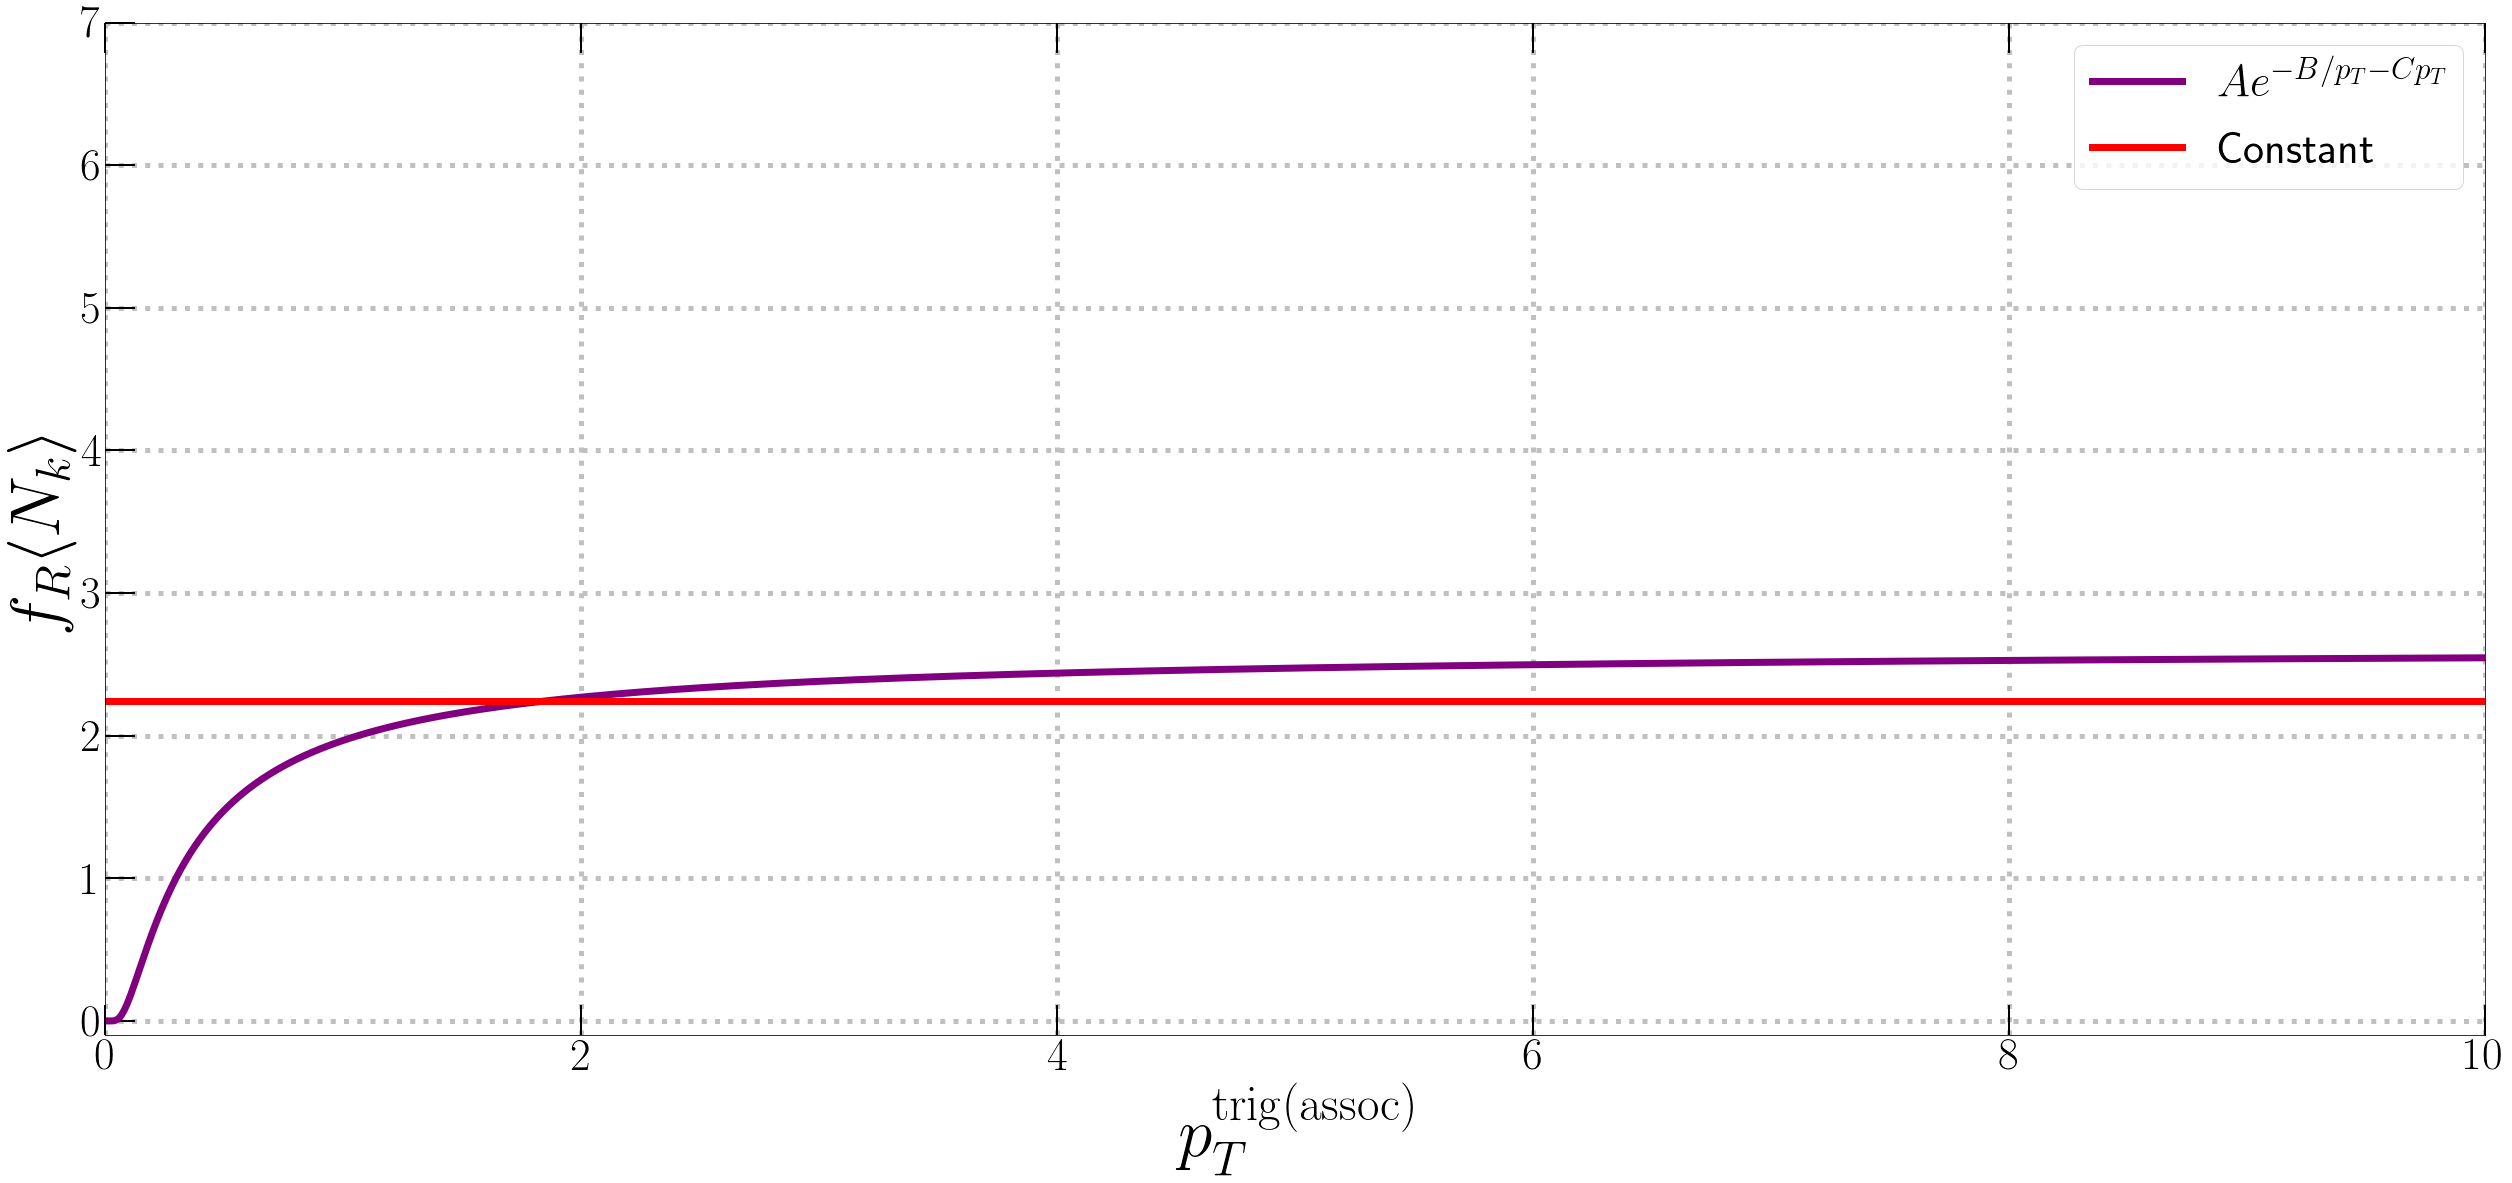
\includegraphics[width=12cm, height=6cm]{./Figures/ptVSnone}
\caption{The $f_R\langle N_k \rangle$ fitting results of $Ae^{-{B} / p_T -C p_{T}}$ form and constant. The purple line is the fitting results of $f_R\langle N_k \rangle = Ae^{-{B} / p_T -C p_{T}}$, and the red line is the fitting result of $f_R\langle N_k \rangle$ as constant. }
\label{figure:ptVSnone}
\end{figure}

Since two results are different only at the $0.1<p_T<1$GeV range in the \ref{figure:ptVSnone}, we use $f_R\langle N_k \rangle$ as constant.


\subsection{Comparing ridge component parameters with previous results}
\label{subsec: comparing parameter}


We compare physical parameters in the ridge component of Momentum-Kick model at STAR AuAu at 200GeV\cite{Wong_1}, CMS PbPb at 2.76TeV\cite{PbPb} and pp at 13TeV, in which ALICE, CMS and ATLAS data are used from reference\cite{alice, cms, atlas}. Parameters of ridge component are summarized in Table \ref{table:param}.

\begin{table}[ht]
  \centering
  \begin{tabular}{C{2cm} | C{2.5cm}  C{3.5cm}  C{2.5cm}  C{2.5cm}  C{2.5cm}}
   \hline \\[-1 ex]
    & AuAu 200 GeV & PbPb 2.76 TeV & pp 13 TeV\cite{Hanul} & pp 7 TeV & pp 13 TeV\\ [1 ex] \hline\hline \\[-1.5 ex]
   T (GeV) & 0.5 & 0.6 & 1.54 & 1.16 & 1.18\\[1ex]
   q (GeV) & 1.0 & 0.7 & 2 & 1.33 & 1.00\\ [1ex]
  $f_R \langle N_k \rangle$ & 4 & $20.2e^{-{1.395} / {\langle p_{T}^{\text{trig}} \rangle}-0.207{\langle p_{T}^{\text{trig}} \rangle}}$ & 0.93, 1.37 & 0.99 & 2.24\\[1.5ex]
   \hline
 \end{tabular}
 \caption{Previous results of the physical parameters in the ridge component of the momentum kick model.}
 \label{table:param}
\end{table}

Since pp at 7 TeV data isn't sufficient compared to pp at 13 TeV, we set the temperature of 7 TeV as a ratio of $\langle p_T \rangle$ and it is expressed as:

\begin{equation} \label{equation:Tempratio}
T_{7 \text{Tev}} = T_{13 \text{Tev}} \times \frac{\langle p_T \rangle_{7 \text{TeV}}}{\langle p_T \rangle_{13 \text{TeV}}}
\end{equation}

And we set $\langle p_T \rangle _{13 \text{TeV}} = $
% 이 부분은 '이 논문에서 이렇게 해석했었다' 라는 형태로 변경하는중.
% 현재, 각 파라미터에 대해서 비교하는중 -> 실험결과별로 변경하는중
% ex) PbPb 2.76 TeV 는 AuAu 200 GeV에 비해서 T는 어떻게...q는 어떻게...

Since $T$ increases as the center of mass energy gets bigger, $T$ becomes higher from 0.5 GeV at AuAu to 0.6 GeV at PbPb. 
For the same reason, $T$ is 1.08 GeV at pp collision at 13 TeV, which is 54.29\% higher than PbPb at 2.76TeV.
Since the 7 TeV has low center of mass energy than 13 TeV, $T$ at the pp collision at 7 TeV is -53.7\% lower than the pp at 13 TeV.

Since the medium density from PbPb is expected to be denser than that from AuAu, the number of kicks between medium partons is higher.
Therefore, the average of momentum transfer per kick in PbPb is lower than in AuAu, as can be seen, $1.0 \rightarrow 0.7$ GeV in Table \ref{table:param}.
However, the medium from pp at 13TeV is expected less dense than that from PbPb, even though the center of mass energy is higher,
$q$ becomes higher from 0.7 GeV at PbPb collision to 0.799 GeV at pp collision. 

Since the initial parton momentum distribution is normalized, $f_R \langle N_k \rangle$ describe the number of particles, which survives and is detected at the detector. We set $f_R \langle N_k \rangle = Ae^{-{B} / {p_{T}} - Cp_T}$ form (A, B, and C are positive real number),
which is the same $f_R \langle N_k \rangle$ form in PbPb at 2.76TeV result\cite{PbPb}.
However, the least square method via the Levenberg-Marquardt algorithm eliminates $e^{-Cp_T}$ term .
Since the pp collision create low density, the number of collisions of particles independent on their momentum, only survival ratio has momentum dependence.
Fig.\ref{figure:frnk} is a graph compared with references\cite{Wong_1, PbPb, Hanul}.


\begin{figure}[ht]
\centering
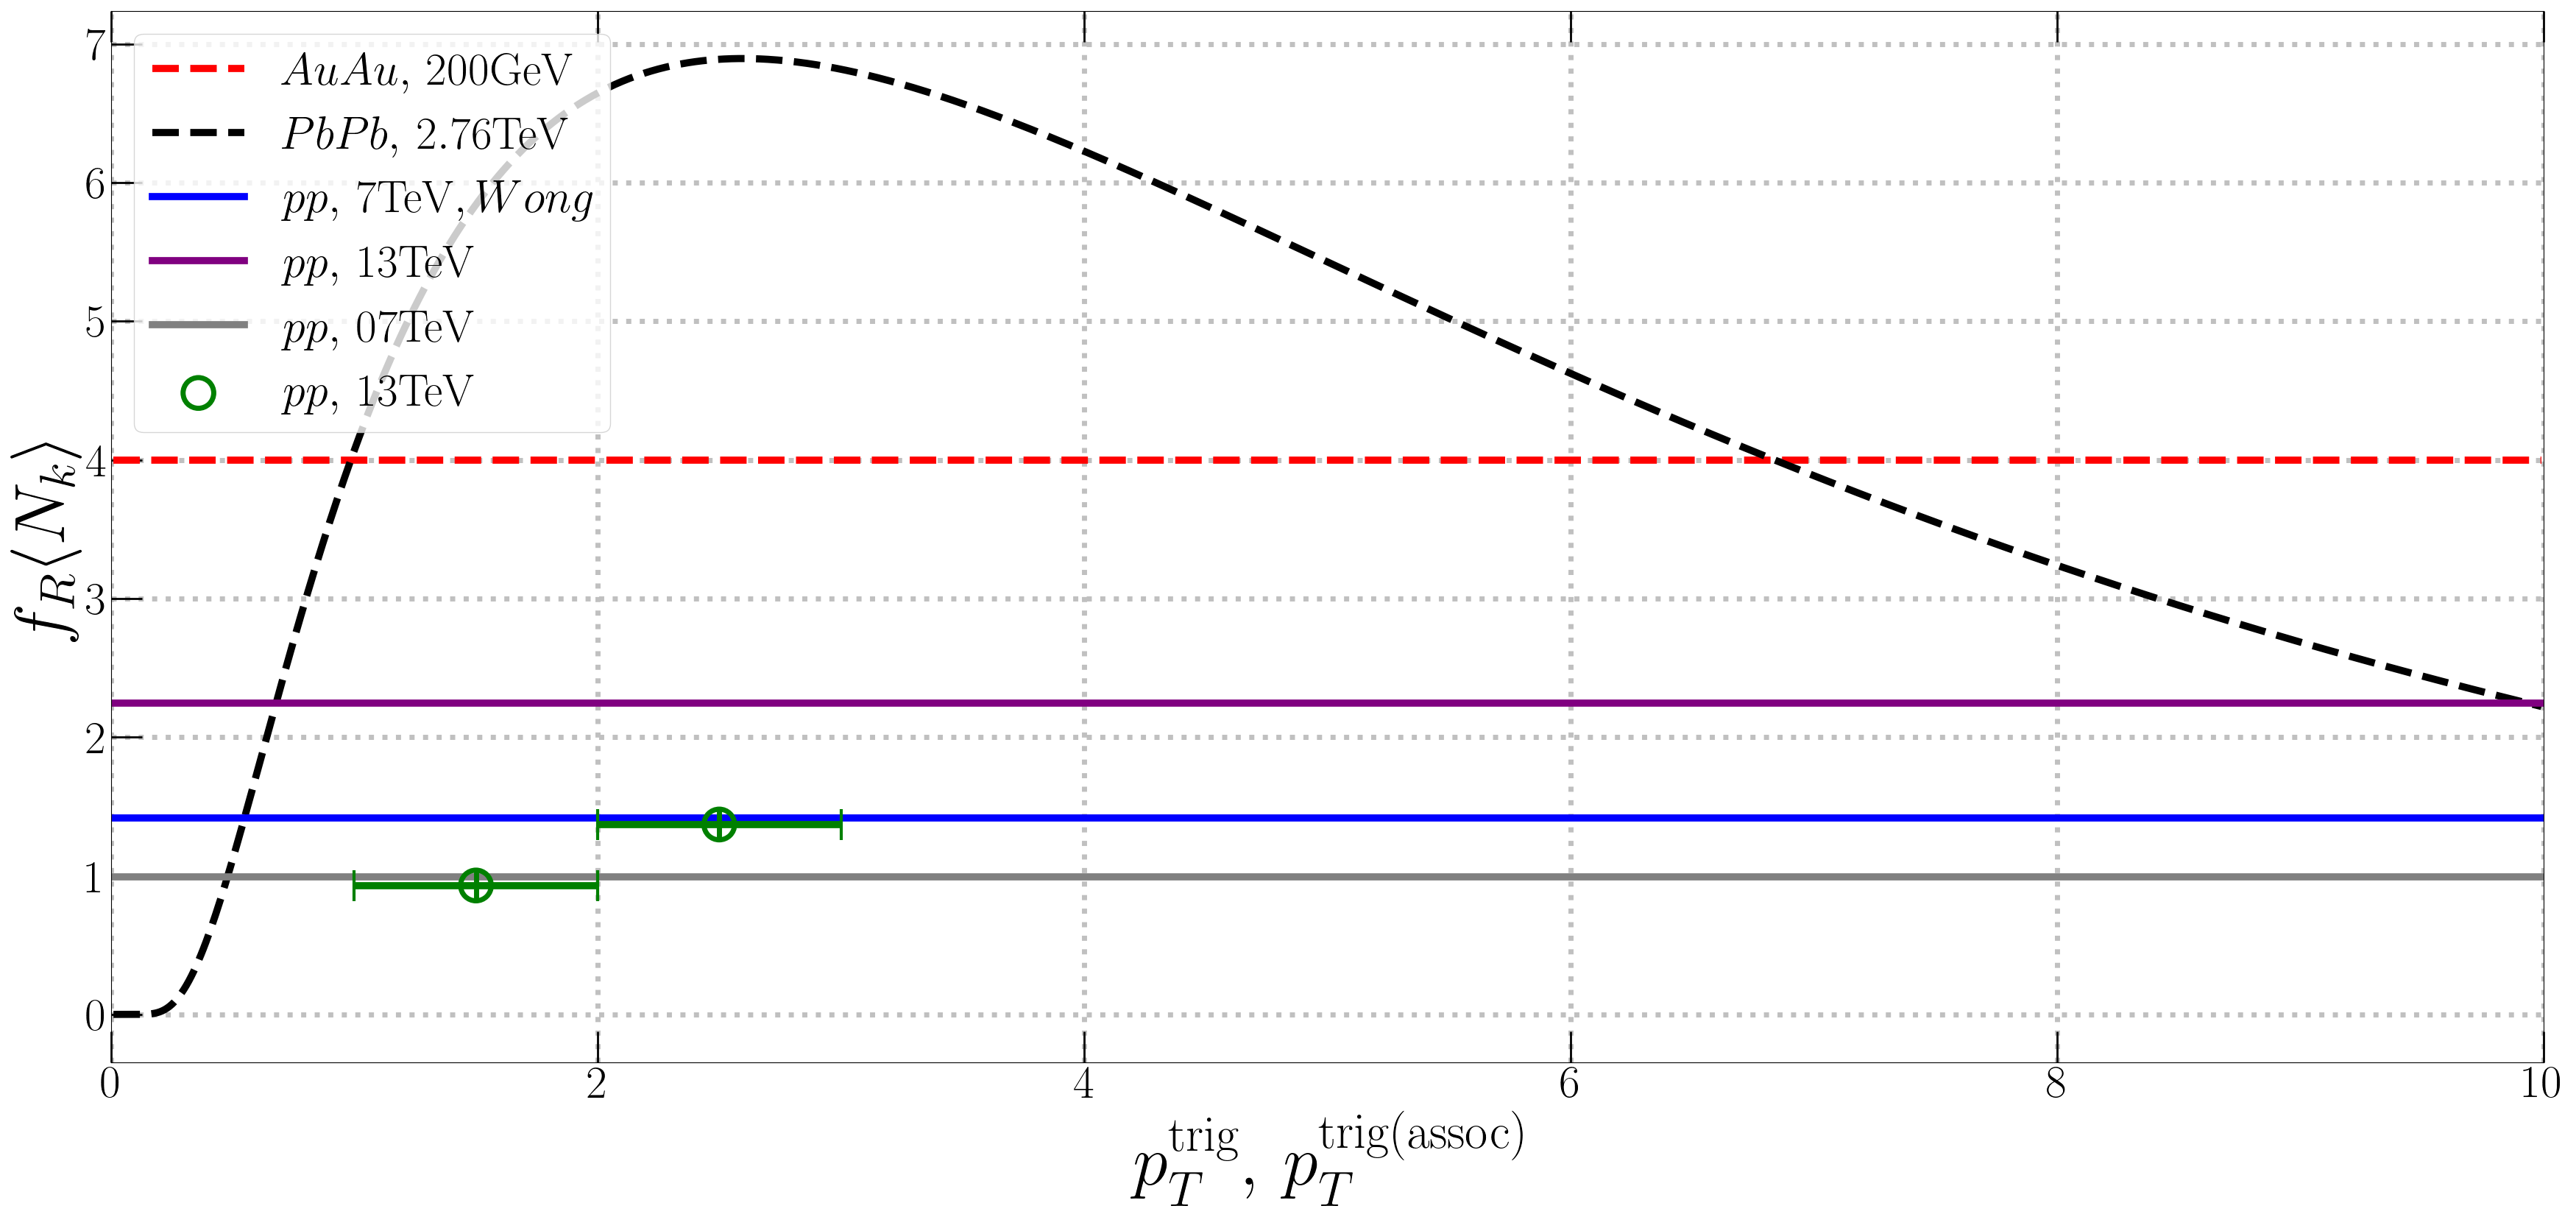
\includegraphics[width=12cm, height=6cm]{./Figures/Paper_frnk}
\caption{The shape of $f_R \left\langle N_k \right\rangle$ in AuAu at 200GeV, PbPb at 2.76TeV and pp at 13TeV for $p_{T}^{trig}$.
Solid line of blue color is result of least square fitting with same form in the reference\cite{PbPb} result and green plots are the results in the reference\cite{Hanul}.}
\label{figure:frnk}
\end{figure}

The PbPb at 2.76 TeV and pp at 13TeV show the results in several bins for $p_T^{\text{trig}}$, and the range of $p_T^{\text{assoc}}$ is only split equal to $p_T^{\text{trig}}$ in the pp at 13TeV. However, we can see the trend.


In the case of AuAu collision at 200GeV, since it has low energy, $f_R \langle N_k \rangle$ doesn't have $p_T$ dependence.
The reference\cite{PbPb} decided  $f_R \langle N_k \rangle$, which has $\langle p_T^{trig} \rangle$ dependence. Since PbPb at 2.76 TeV has high energy and creates high medium density, $f_R$ has exponentially increase and $\langle N_k \rangle$ has exponentially decrease as $\langle p_T^{\text{trig}} \rangle$. This is because, the particles, which are the high-range of $p_T$, can survive easily, but the number of kicked medium partons gets lower.
However, in pp collision, because of lower density, the high-range of $p_T$ can easily survive, but the number of kicked medium partons is maintained.

We fit the Momentum-Kick model as a least square method to the ALICE and CMS proton-proton collision 13TeV at high-multiplicity\cite{alice, cms}, and we also draw the ATLAS high-multiplicity pp collision results\cite{atlas}.

\begin{figure}[ht]
\centering

\includegraphics[width=18cm, height=3cm]{./Figures/Paper_phiCorr}
\caption{Result for $\Delta \phi$ correlation. All curves are momentum kick model result, plots are experimental data.
Red is the result from ALICE, black is from CMS and blue is from ATLAS.
For ALICE and CMS data, we draw the case of $1<p_T<2, 2<p_T<3, 3<p_T<4$, and we also draw $0.1<p_T<1$ case for CMS data. And in ATLAS data, we draw for $0.5<p_T<5$.}
\label{figure:phicorr}
\end{figure}

\begin{figure}[ht]
\centering
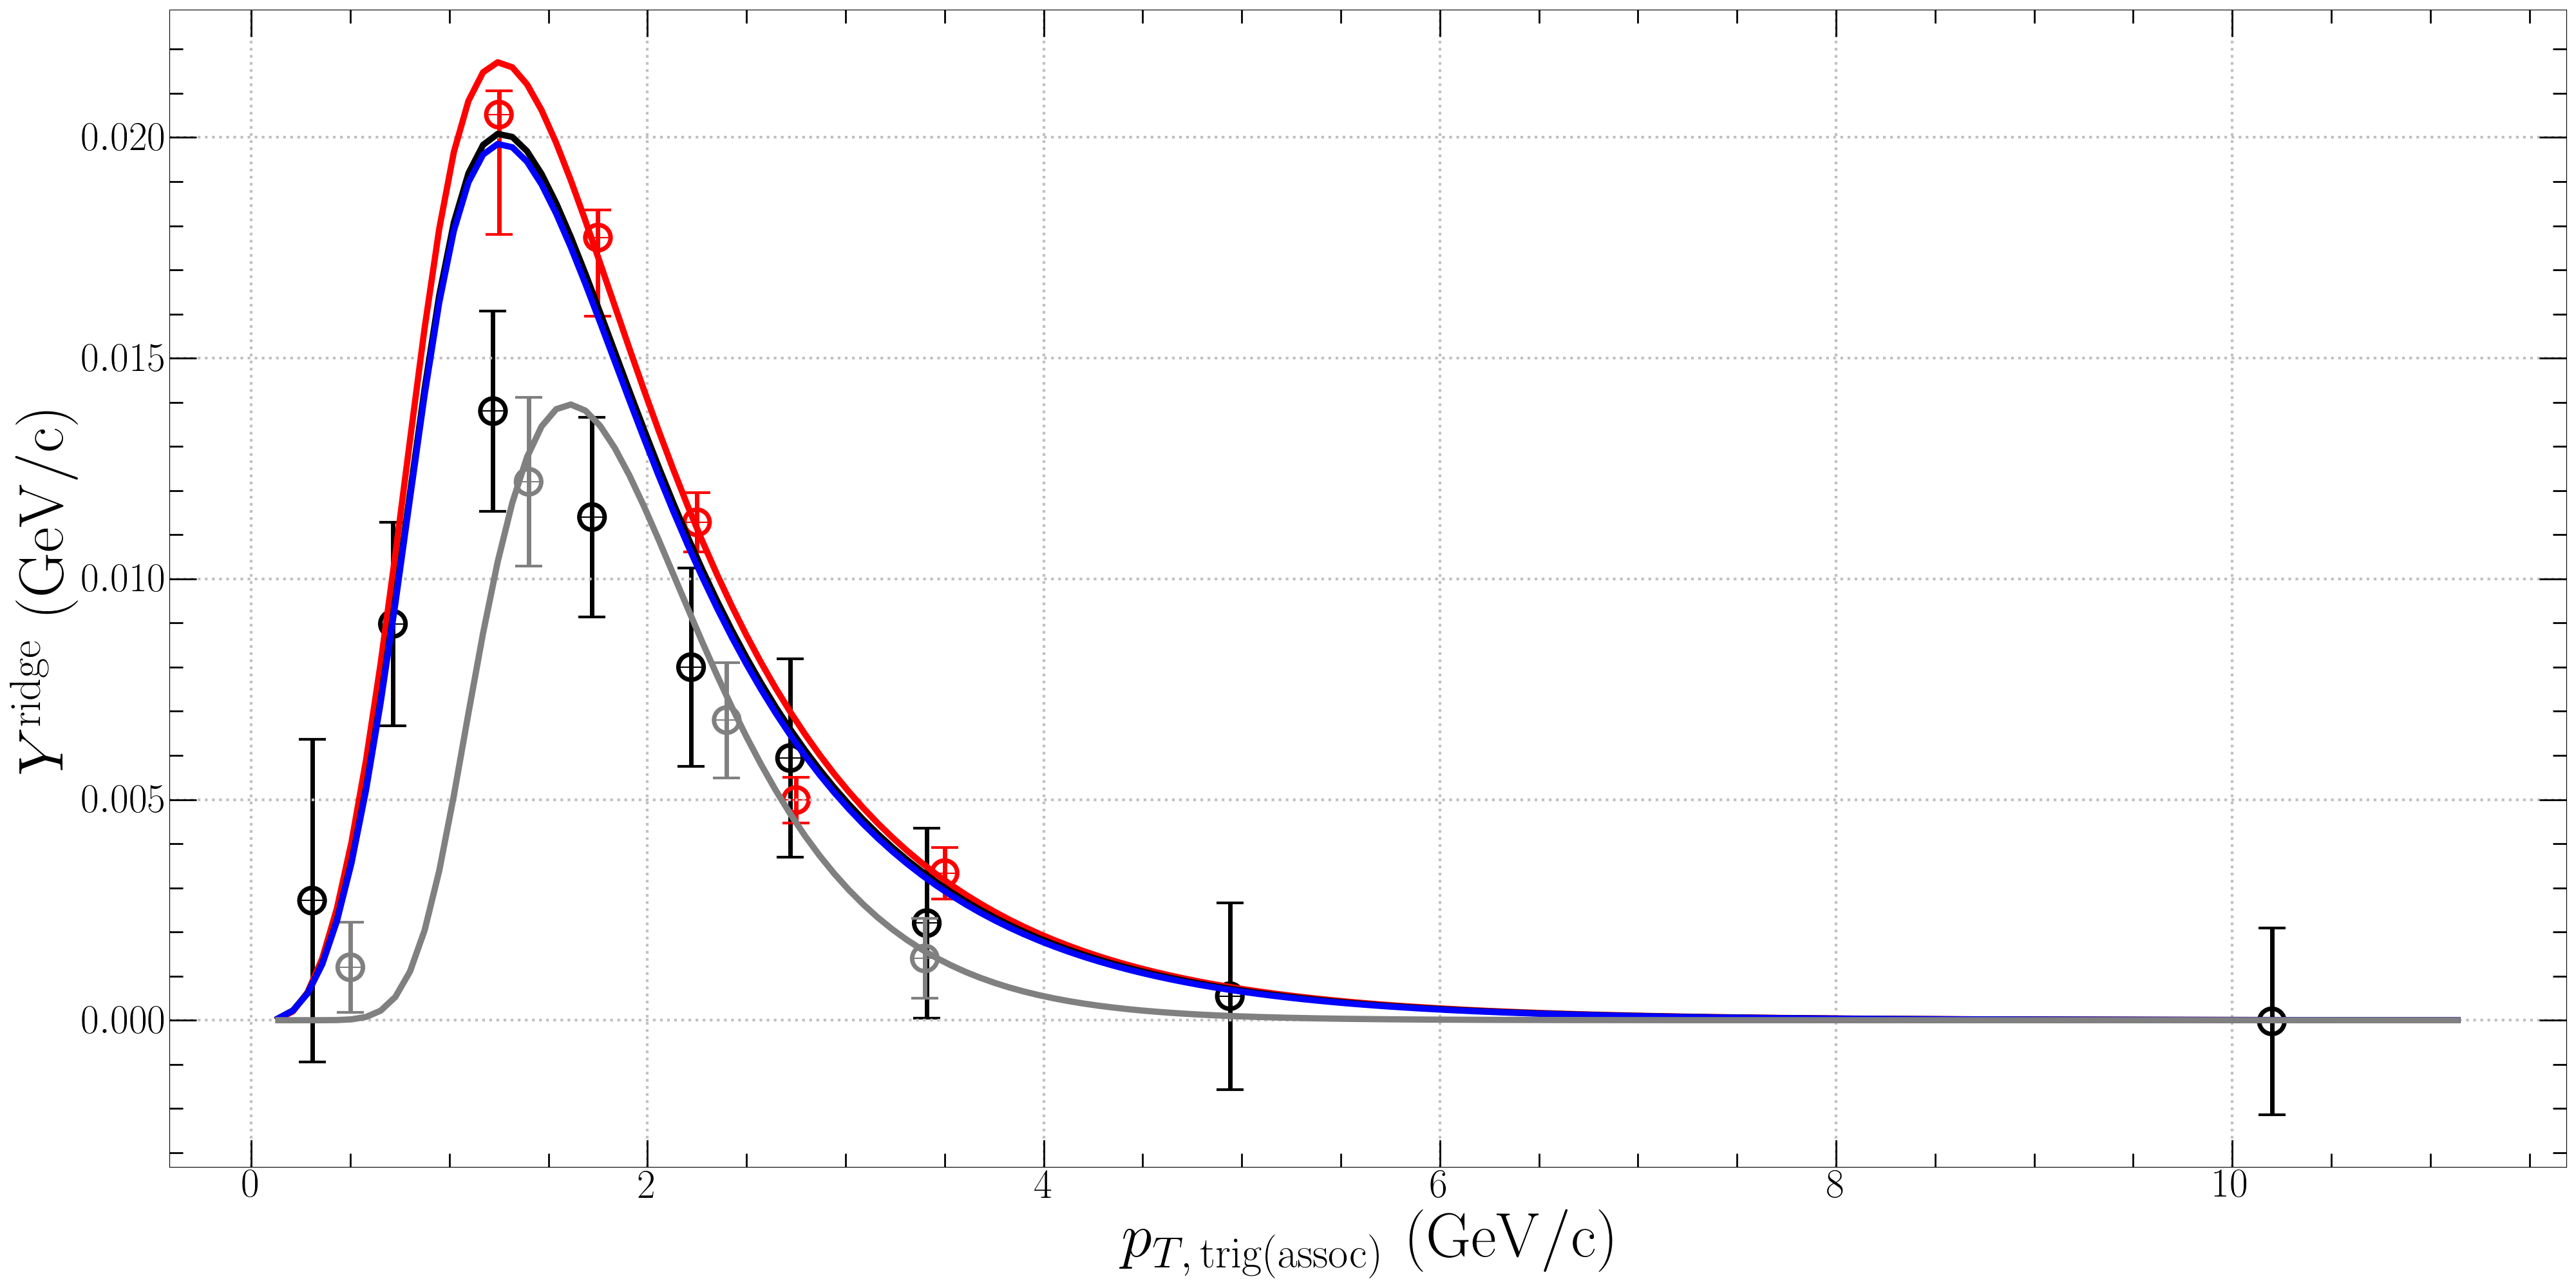
\includegraphics[width=12cm, height=6cm]{./Figures/Paper_pTdis}
\caption{Yield for $p_T$ distribution at ALICE and CMS data. We do not include ATLAS data, because they don't supply the results for $p_T$ bins.}
\label{figure:pTdis}
\end{figure}

In Fig. \ref{figure:phicorr} and \ref{figure:pTdis}, we draw Momentum-Kick model results and LHC data together.
The solid line is the Momentum-Kick model results, and the circles are the experimental data.
Red color is ALICE data and Momentum-Kick model results, black is for CMS, and blue is for ATLAS.
In the Fig. \ref{figure:phicorr}, the ATLAS collaboration's data is significantly higher than others.
This is because, they didn't normalize as $p_T$ bin, so I also do not normalize either.
Experimental data is well described via Momentum-Kick model for all $p_T$ ranges.
In Fig. \ref{figure:pTdis}, since partons are kicked as $\textbf{q}$ by jet particles, the theoretical ridge yield must show a peak at $q$.
% However, since $f_R \langle N_k \rangle $ is proportional to ${p_T}^2$, the position of the peak is moved to an area where the $p_T$ is larger. 
As can be seen in Fig.\ref{figure:pTdis}, the peak is made around $p_T=1.2$GeV.
Overall, the Momentum-Kick model can describe well for the $\Delta\phi$ correlation and $p_T$ distribution yield, too.


\section*{Various multiplicity}
\label{sec:Various multiplicity}

We already know that near-side ridge structure appears in the high multiplicity proton-proton collisions.
So, we have to check the other multiplicity, like the low multiplicity.
The CMS and ATLAS collaboration provide $\Delta \phi$ correlation in the various multiplicity, and the multiplicity distribution.
The reference \cite{Wong_5} and \cite{PbPb} introduced $\langle p_T \rangle$ ratio at the temperature.
We also introduced $\langle p_T \rangle$ ratio at the $T$ in other multiplicity, .
Based on the results of high multiplicity, we fixed temperature in the other multiplicity as the ratio of $\langle p_T \rangle$

Since the CMS multiplicity data have very high fluctuation, I use only ATLAS data.
\begin{figure}[ht]
\centering
\includegraphics[width=15cm, height=15cm]{./Figures/rezero_atlas_Nk.png}
\caption{$\Delta \phi$ correlation with multiplicity dependence data.}
\label{figure:multiplicity}
\end{figure}
    



\section*{CONCLUSIONS}
\label{sec:Conclusion}


We have analyzed the long-range near-side proton-proton collision at $\sqrt{s_\text{NN}}=13$TeV in ALICE, CMS and ATLAS data. 
Since the small system has less flow effect than heavy-ion collision, the Momentum-Kick model is expected to be applied well in the high multiplicity pp collision.
We apply Momentum-Kick model in high multiplicity pp collision at 13TeV data from all 3 collaboration, altogether. 
As a result, we obtain $T=0.841$ GeV, $q=0.799$ GeV, $f_R\left\langle N_k\right\rangle = 6.710e^{-1.494/p_T-3.519\times10^{-12}p_T}$.
Because of higher energy, the medium temperature is 40.167\% higher than PbPb collision.
Also, because the medium from pp collision has less density than heavy-ion collisions, the jet particles kick medium partons less than PbPb collision.
Therefore, the average momentum transfer per kicked medium partons is 14.143\% higher than PbPb collision at 2.76TeV.
We also introduce $p_T$ dependence on $f_R\left\langle N_k\right\rangle$ as in the reference\cite{PbPb}.
Since high density is created in PbPb at 2.76TeV collision, jet particles kick many of initial medium particles as $\textbf{q}$.
Therefore, many of final particles, which is middle range of $p_T$, are created.
As a result, $f_R \langle N_k \rangle$ in PbPb collision has a maximum value at mid-range of $p_T$.
The particles that the high range of $p_T$ can survive easily in the proton-proton collision, it has the same as PbPb collisions.
However, since pp collision at 13TeV makes lower density than PbPb collisions, the number of kicked medium partons is irrelevant to $p_T$.

Furthermore, we expect the Momentum-Kick model can well describe other diverse data.
Therefore, we will try to explain other data, like various multiplicity and center of mass energy, via the Momentum-Kick model.
\bibliography{Bibliography}

\end{document}
